\documentclass{oblivoir}
\usepackage{amsmath,amssymb,amsthm,kotex,mdframed,paralist,kswrapfig}

\newcounter{num}
\newcommand{\prob}
{\bigskip\noindent\refstepcounter{num}\textbf{문제 \arabic{num})}\par}

\newcommand{\ans}{\par{\raggedleft\textbf{답 : (\qquad\qquad\qquad\qquad\qquad\qquad)}
\par}\bigskip}

\newcommand\ga{\text{(가)}}
\renewcommand\na{\text{(나)}}
%%%
\begin{document}
\Large

\title{승재 23 - 6학년 2학기 - 16}
\author{}
\date{\today}
\maketitle
%\tableofcontents

\newpage

\prob
어떤 물건을 원래 가격의 22\%를 인상하여 1830원에 팔았습니다. 원래 가격은 얼마입니까?
\ans

\prob
어떤 물건을 원래 가격의 13\%를 할인하여 3480원에 팔았습니다. 원래 가격은 얼마입니까?
\ans


%
\prob
아래 그림에서 선분 AB와 선분 BD의 길이의 비는 5:13이고 선분 AC와 선분 CD의 길이의 비는 5:4입니다.
선분 BC의 길이가 15cm일 때, 전체 선분의 길이를 구하세요.

\begin{figure}[h!]
\centering
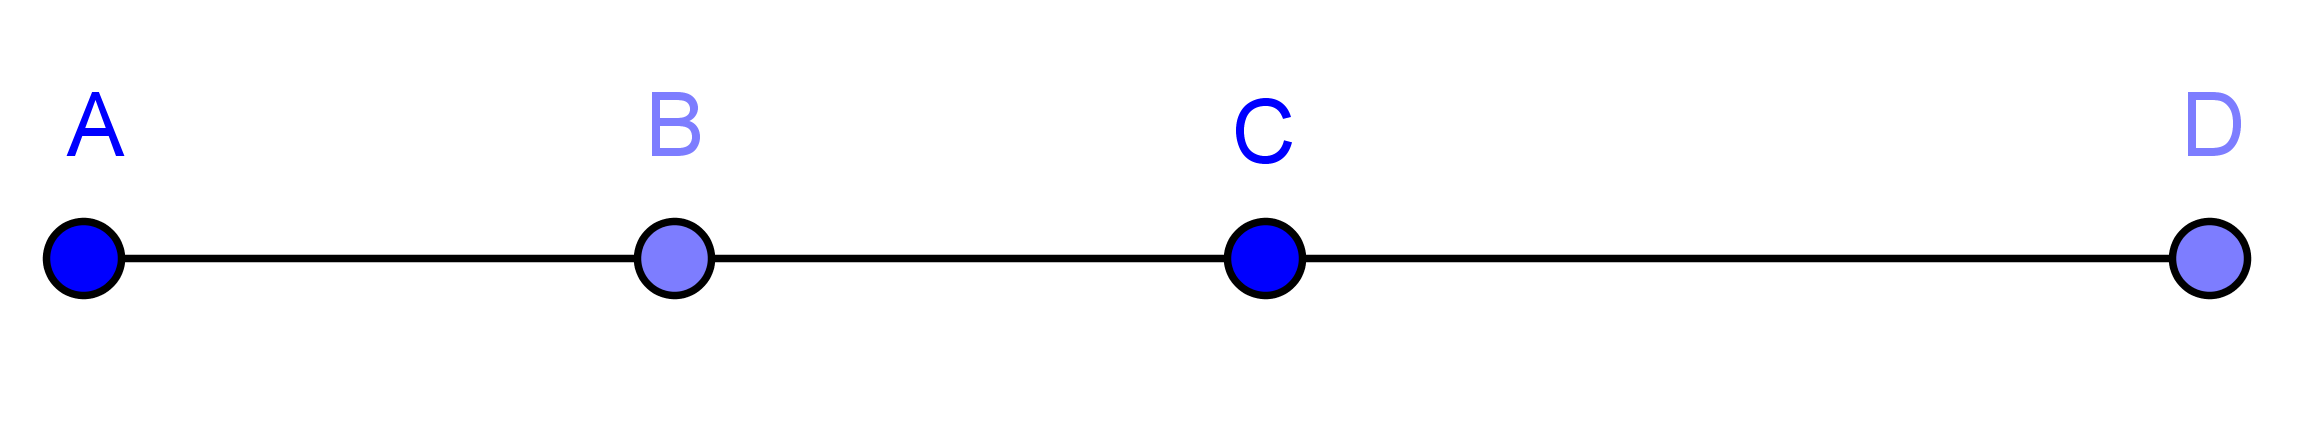
\includegraphics[width=0.5\textwidth]{03}
\end{figure}
\ans

%
\prob
아래 그림에서 선분 AB와 선분 BD의 길이의 비는 2:7이고 선분 AC와 선분 CD의 길이의 비는 5:1입니다.
선분 BC의 길이가 5.5cm일 때, 전체 선분의 길이를 구하세요.
\begin{figure}[h!]
\centering
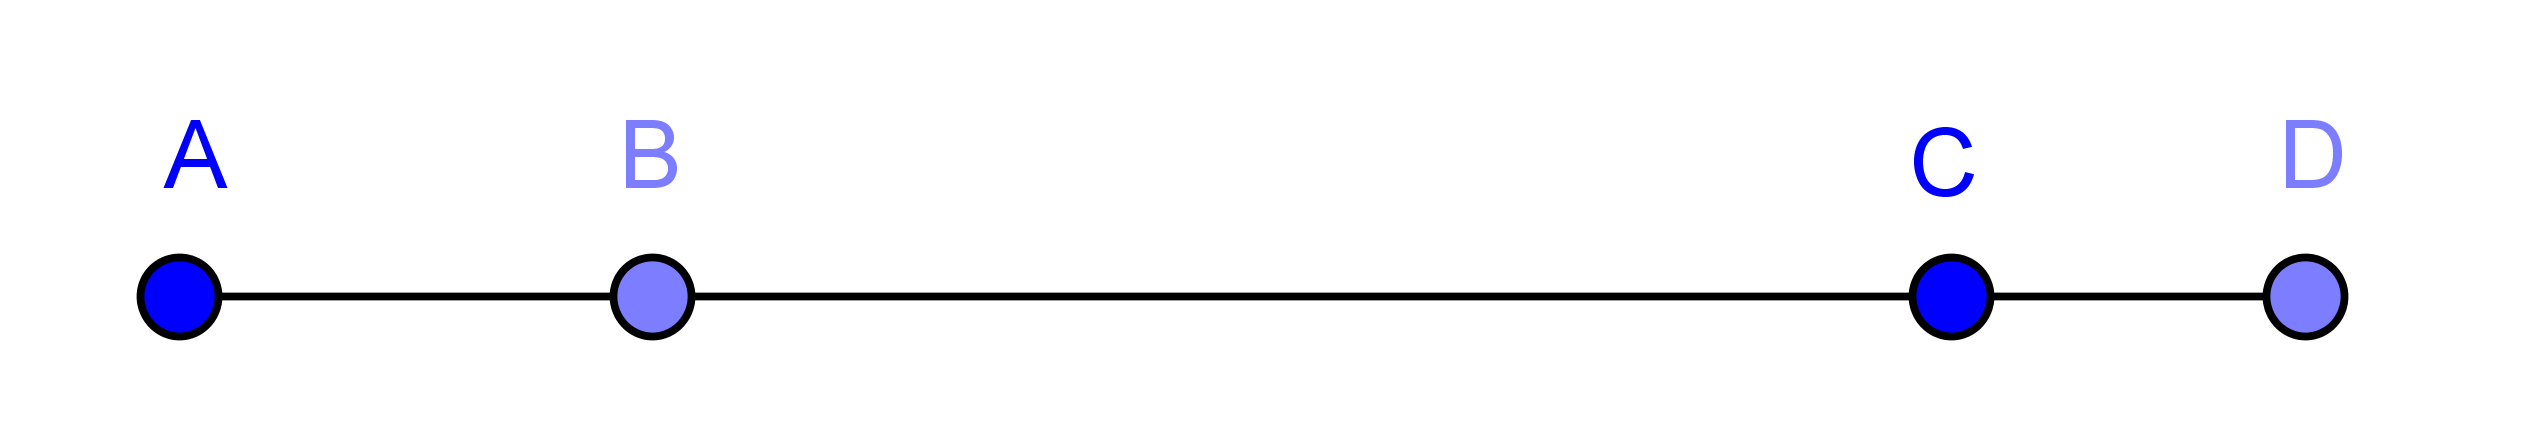
\includegraphics[width=0.5\textwidth]{04}
\end{figure}
\ans

\newpage

%
\prob
사랑이네 학교 학생들이 좋아하는 계절을 조사하여 나타낸 띠그래프입니다.
봄을 좋아하는 학생은 99명이고, 봄을 좋아하는 학생 수는 여름을 좋아하는 학생 수의 75\%일 때, 사랑이네 학교 학생 수는 모두 몇 명입니까?
\begin{figure}[h!]
\centering
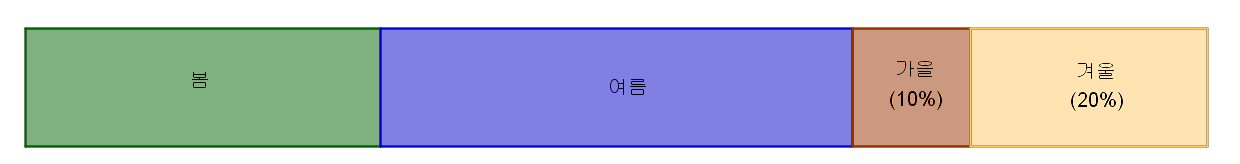
\includegraphics[width=0.9\textwidth]{05}
\end{figure}
\ans

%
\prob
사랑이네 학교 학생들이 좋아하는 계절을 조사하여 나타낸 띠그래프입니다.
봄을 좋아하는 학생은 30명이고, 봄을 좋아하는 학생 수는 여름을 좋아하는 학생 수의 40\%일 때, 사랑이네 학교 학생 수는 모두 몇 명입니까?
\begin{figure}[h!]
\centering
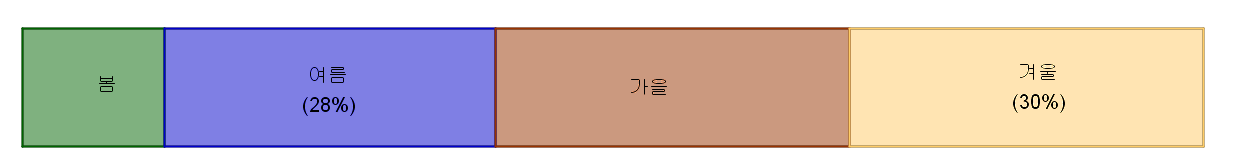
\includegraphics[width=0.9\textwidth]{06}
\end{figure}
\ans

\newpage

%
\prob
아래 그림과 같이 직사각형 (가)와 (나)가 겹쳐져 있습니다.
겹쳐진 부분의 넓이는 (가)의 넓이의 \(30\%\)이고, (나)의 넓이의 \(\frac14\)입니다.
직사각형 (가)와 (나)의 넓이의 비를 가장 간단한 자연수의 비로 나타내세요.
\begin{figure}[h!]
\centering
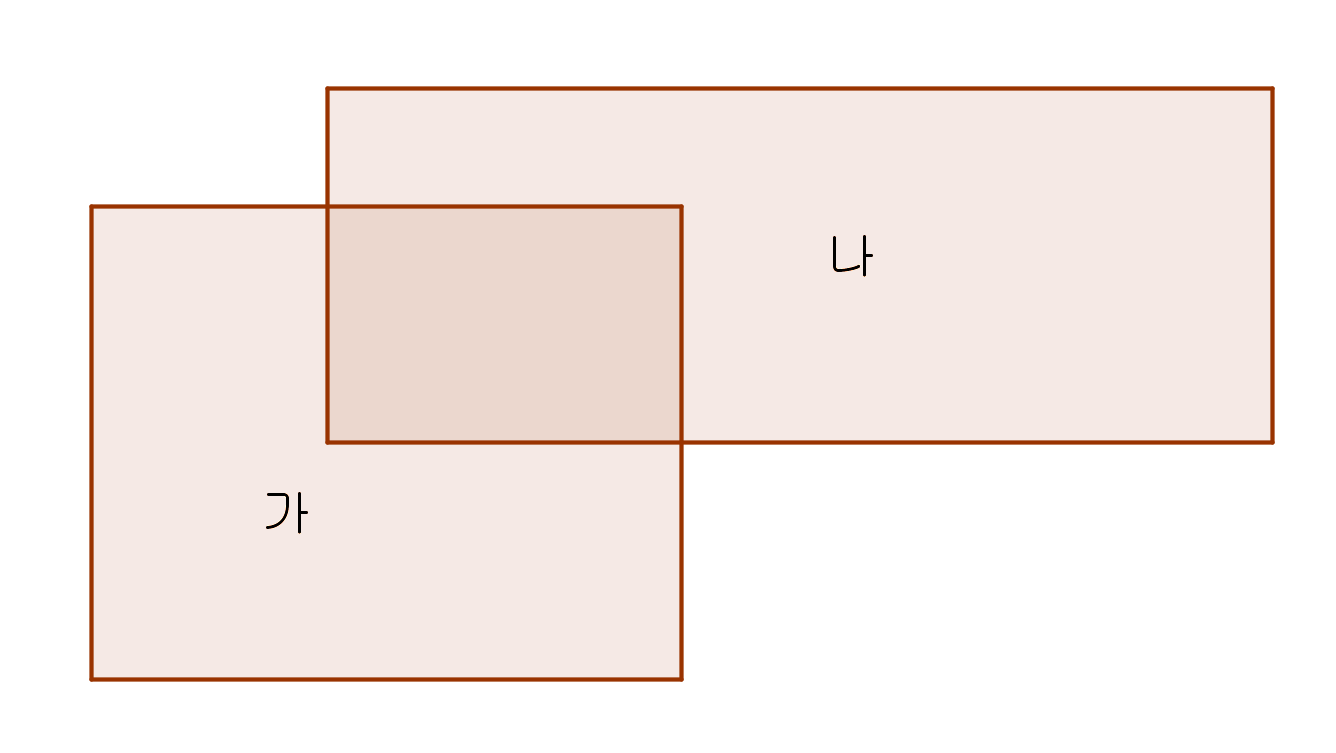
\includegraphics[width=0.5\textwidth]{07}
\end{figure}
\ans

%
\prob
아래 그림과 같이 겹쳐진 두 직사각형 (가)와 (나)의 넓이의 비가 21:25 입니다.
겹쳐진 부분의 넓이는 (가)의 넓이의 \(\frac27\)일 때, 겹쳐진 부분의 넓이는 직사각형 (나)의 넓이의 몇 \%입니까?
\begin{figure}[h!]
\centering
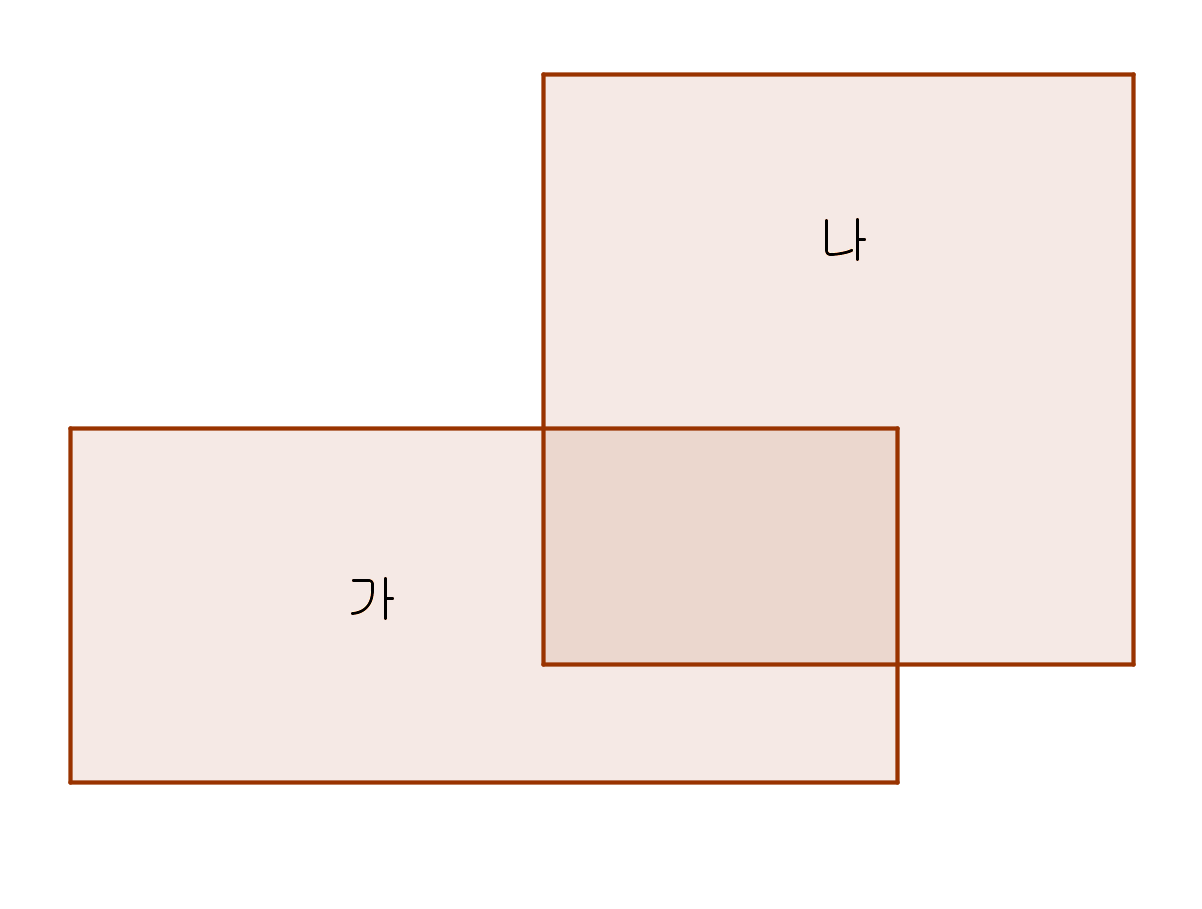
\includegraphics[width=0.5\textwidth]{08}
\end{figure}
\ans

\newpage

%
\prob
다음 그림과 같이 A, B 두 개의 원기둥이 있습니다.
1m를 굴러가는데 A는 20바퀴 회전하였고 B는 15바퀴 회전했습니다.
A, B의 밑면의 반지름의 비를 구하세요.

\begin{figure}[h!]
\centering
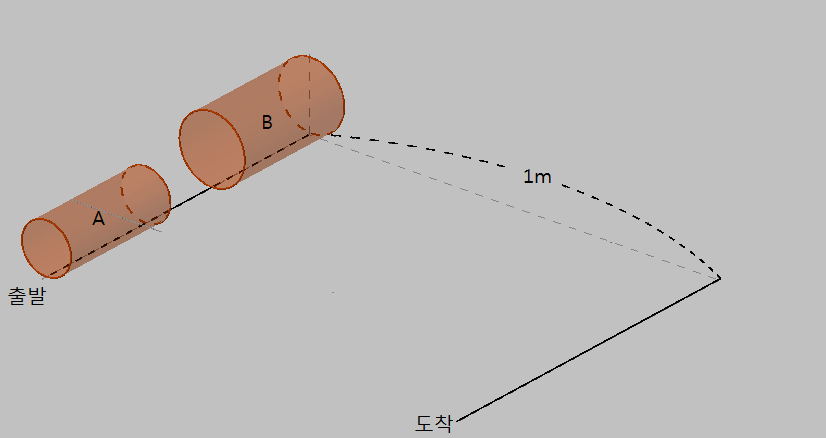
\includegraphics[width=0.7\textwidth]{09}
\end{figure}

\begin{mdframed}
\textbf{풀이 : }
\vspace{0.2\textheight}
\end{mdframed}
\ans

\newpage

%
\prob
준호가 이번 시험에서 받은 국어, 영어, 수학 점수를 살펴보았더니, 국어 점수는 영어 점수의 \(\frac67\)이고 수학 점수는 국어 점수의 \(\frac65\)이었습니다.
이 때, 수학 점수:영어 점수를 가장 간단한 자연수의 비로 나타내고, 그 풀이과정을 쓰세요.

\begin{mdframed}
\textbf{풀이 : }
\vspace{0.2\textheight}
\end{mdframed}
\ans

%
\prob
상재의 영어 점수는 국어 점수의 1.125이고 수학 점수는 영어 점수의 1.5입니다.
이 때, 수학 점수:국어 점수를 가장 간단한 자연수의 비로 나타내고, 그 풀이과정을 쓰세요.

\begin{mdframed}
\textbf{풀이 : }
\vspace{0.2\textheight}
\end{mdframed}
\ans

\newpage

%
\prob
(가)의 0.2는 (나)의 \(\displaystyle\frac14\)과 같을 때 (가) : (나)를 가장 간단한 자연수의 비로 나타내고, 그 풀이과정을 쓰세요.
\begin{figure}[h]
\centering
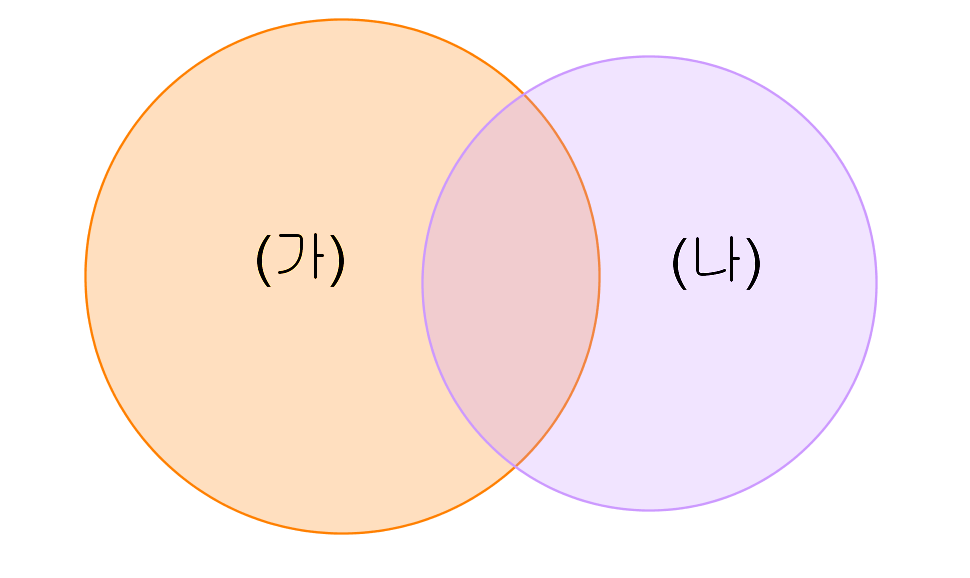
\includegraphics[width=0.5\textwidth]{venn}
\end{figure}
\begin{mdframed}
\textbf{풀이 : }
\vspace{0.15\textheight}
\end{mdframed}

%
\prob
(가) : (나)를 가장 간단한 자연수의 비로 나타내고 그 풀이과정을 쓰세요.
\[
\ga\times\frac38=\na\times0.7
\]
\begin{mdframed}
\textbf{풀이 : }
\vspace{0.15\textheight}
\end{mdframed}
\ans

\newpage


%
\prob
가로, 세로, 높이의 비가 2:3:6인 직육면체가 있습니다.
이 직육면체의 모서리의 길이의 합이 121cm일 때, 이 직육면체의 부피를 구하세요.
\begin{figure}[h!]
\centering
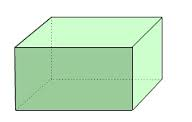
\includegraphics{parallelopipedon}
\end{figure}
\ans

\newpage

%
\prob
지호와 영신이는 사과 두 개를 먹었습니다.
지호와 영신이가 먹은 사과의 양을 가장 간단한 자연수의 비로 나타내세요.
\ans

\begin{figure}[h!]
\centering
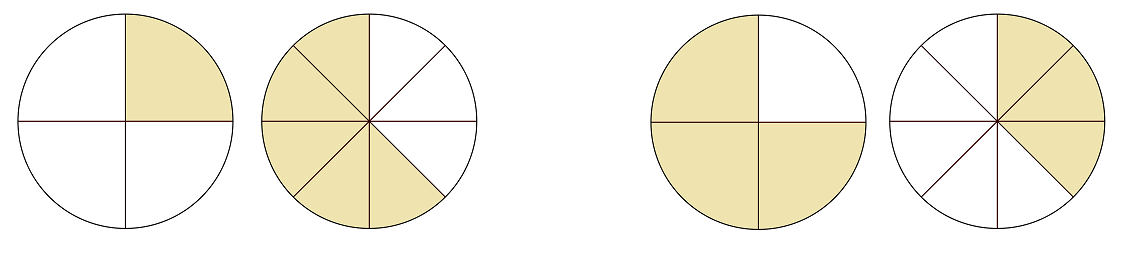
\includegraphics[width=0.9\textwidth]{020}

지호가 먹은 사과\qquad\qquad\qquad\qquad\quad 영신이가 먹은 사과
\end{figure}

%
\prob
지수와 효정이는 사과 두 개를 먹었습니다.
지수와 효정이가 먹은 사과의 양을 가장 간단한 자연수의 비로 나타내세요.
\ans
\begin{figure}[h!]
\centering
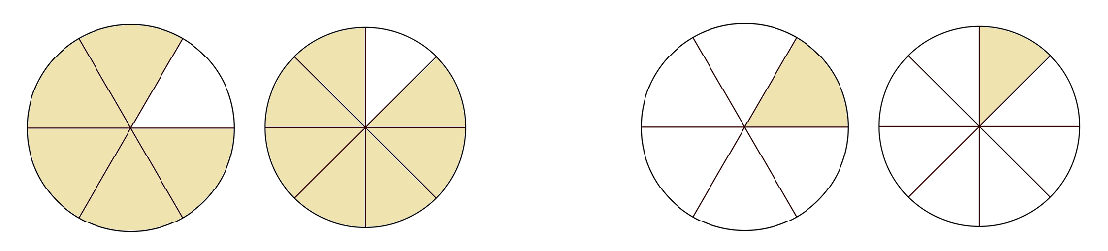
\includegraphics[width=0.9\textwidth]{030}

지수가 먹은 사과\qquad\qquad\qquad\qquad\quad 효정이가 먹은 사과
\end{figure}


\newpage

%
\prob
같은 크기의 옆면으로 만든 서로 다른 원기둥의 부피를 구하려고 합니다.
물음에 답하세오.
(원주율:3.1)
\begin{figure}[h!]
\centering
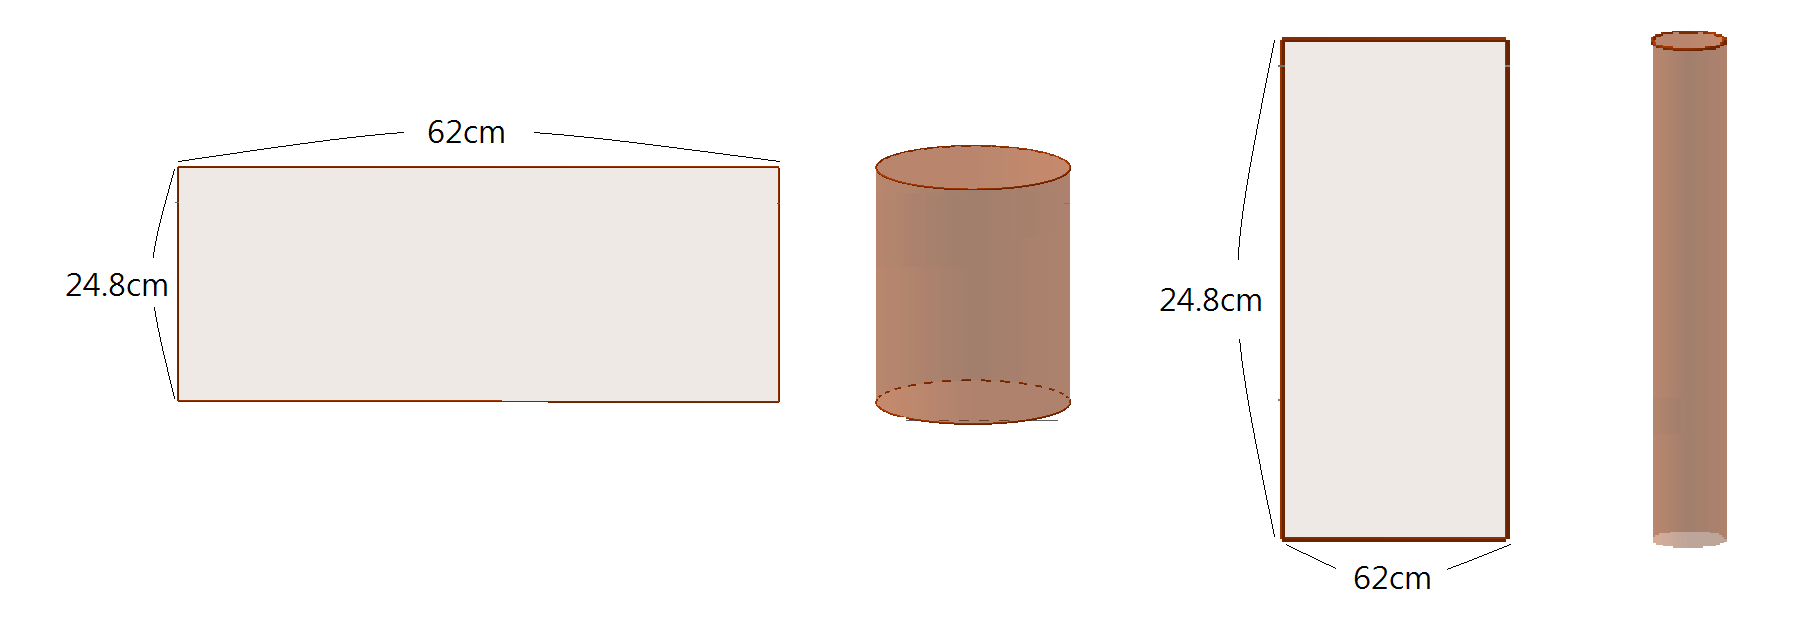
\includegraphics[width=0.9\textwidth]{17}
\end{figure}

(1) 직사각형 `가'를 옆면으로 하여 만든 원기둥의 부피는 몇 cm\(^3\) 입니까?

\ans

(2) 직사각형 `나'를 옆면으로 하여 만든 원기둥의 부피는 몇 cm\(^3\) 입니까?

\ans

\newpage
\prob
다음 그림에서 선분 BH의 길이를 구하세요.
\begin{figure}[h!]
\centering
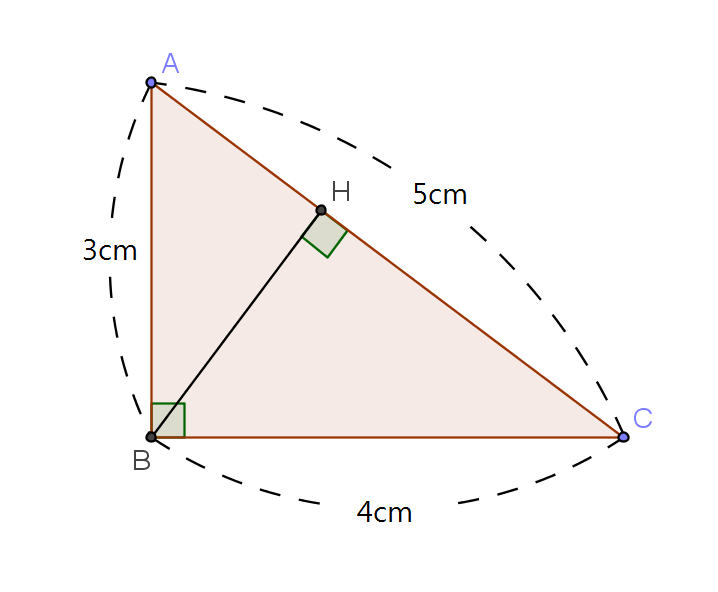
\includegraphics[width=0.7\textwidth]{18}
\end{figure}

\ans

\prob
다음 그림에서 선분 AC의 길이를 구하세요.
(선분 DH는 \(\frac{60}{13}\)cm입니다.)
\begin{figure}[h!]
\centering
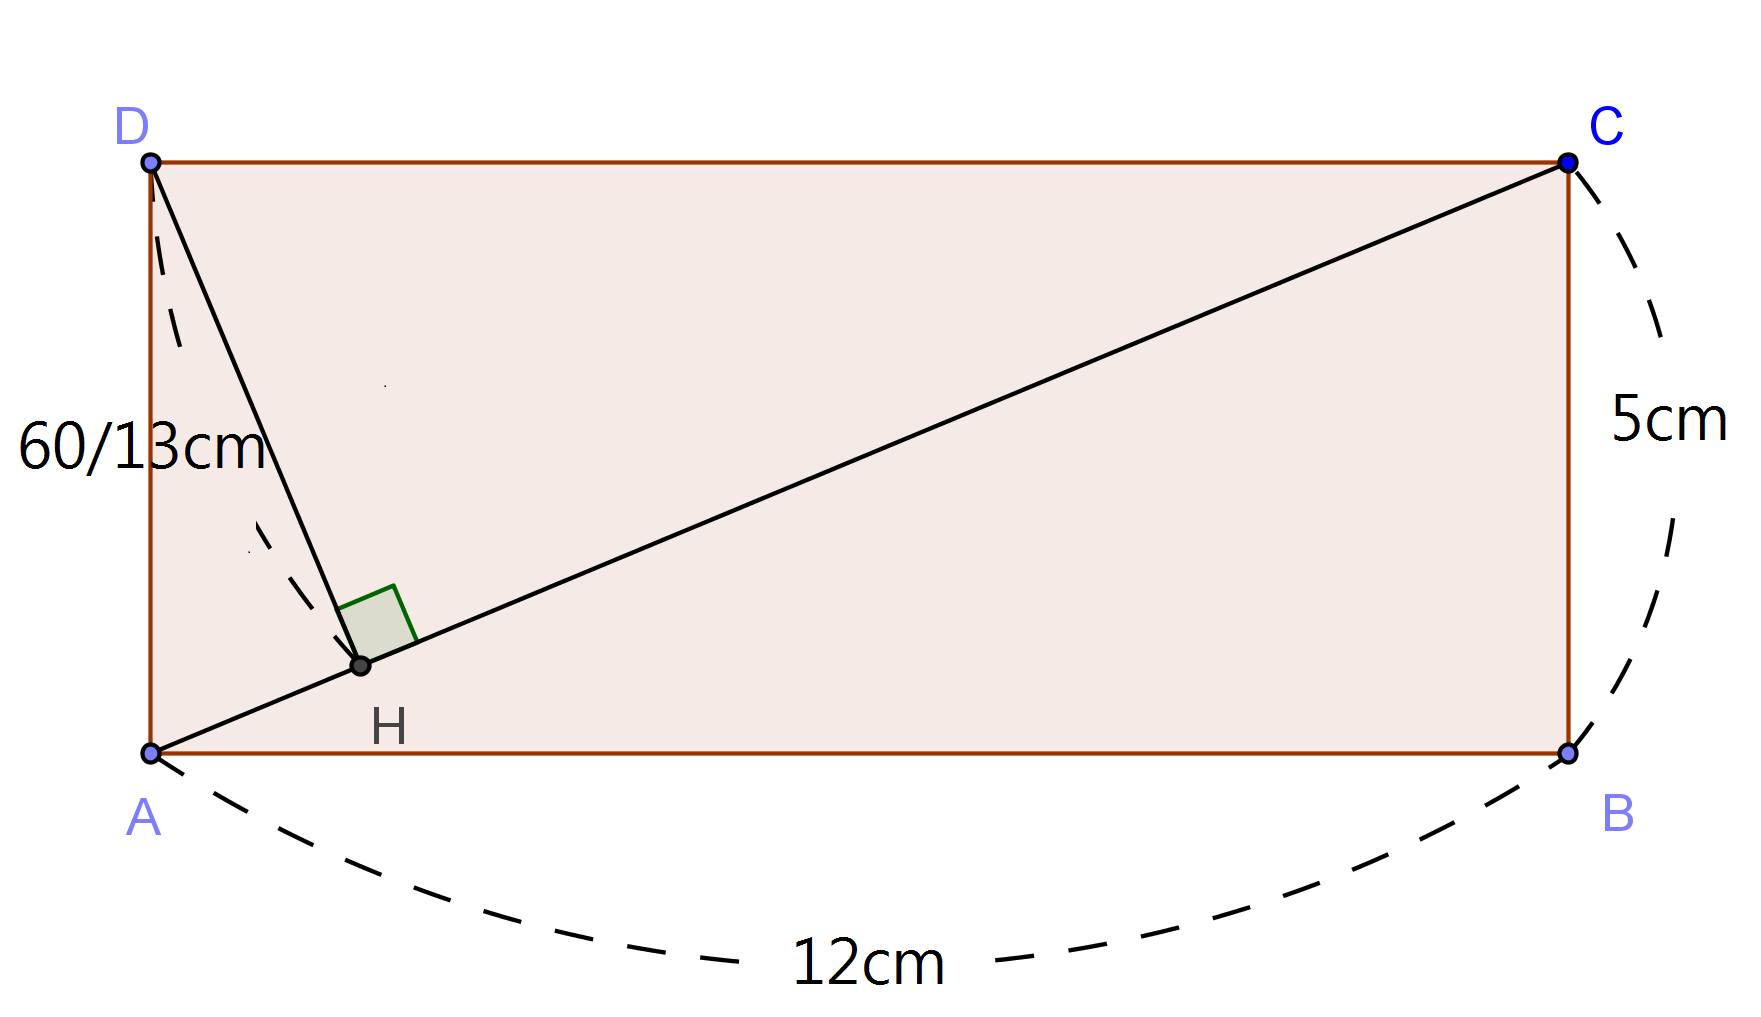
\includegraphics[width=0.7\textwidth]{19}
\end{figure}

\ans

\newpage
\prob
소영이네 6학년 학생 수는 280명입니다.
이 중 김치찌개를 좋아하는 학생은 전체의 40\%이고, 부추전을 좋아하는 학생은 전체의 35\%입니다.
김치찌개와 부추전을 좋아하는 학생은 전체의 20\%일 때, 김치찌개도 싫어하고, 부추전도 싫어하는 학생은 전체의 몇 \%입니까?
\ans

\prob
동락이네 6학년 학생 수는 320명입니다.
이 중 콜라를 좋아하는 학생은 전체의 65\%이고, 사이다를 좋아하지 않는 학생은 전체의 70\%입니다.
콜라와 사이다를 모두 좋아하는 학생은 전체의 25\%일 때, 콜라는 좋아하지만, 사이다는 좋아하지 않는 학생은 전체의 몇 \%입니까?
\ans

\prob
기훈이네 6학년 학생 수는 180명입니다.
이중 원피스를 좋아하는 학생은 전체의 30\%이고, 드래곤볼을 좋아하는 학생은 전체의 25\%입니다.
원피스와 드래곤볼을 모두 좋아하지 않는 학생이 전체의 70\%일 때, 원피스와 드래곤볼을 모두 좋아하는 학생은 전체의 몇 \%입니까?
\ans




\end{document}